\documentclass{article}
\usepackage{tikz}
\usetikzlibrary{decorations.markings}

\begin{document}
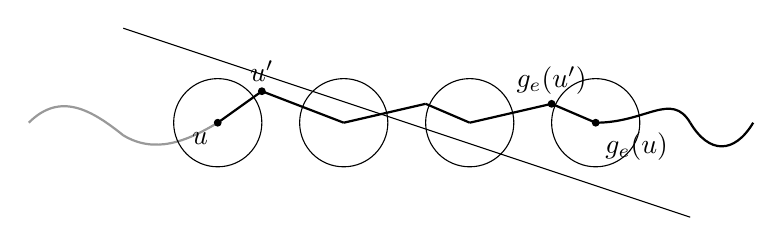
\begin{tikzpicture}[scale=0.8]
    % Define colors
    \colorlet{walkgray}{gray!80}
    
    % Draw the original walk (gray part)
    \draw[walkgray, thick] (-5,0) .. controls (-4.5,0.5) and (-4,0.2) .. (-3.5,-0.2);
    
    % Draw the splitting point and continuation
    \draw[walkgray, thick] (-3.5,-0.2) .. controls (-3,-0.5) and (-2.5,-0.3) .. (-2,0);
    
    % Draw circles representing boundaries
    \draw[thin] (-2,0) circle (0.7);
    \draw[thin] (0,0) circle (0.7);
    \draw[thin] (2,0) circle (0.7);
    \draw[thin] (4,0) circle (0.7);
    
    % Draw the modified walk (black part)
    \draw[thick] (-2,0) -- (-1.3,0.5);
    \draw[thick] (-1.3,0.5) -- (0,0);
    \draw[thick] (0,0) -- (1.3,0.3);
    \draw[thick] (1.3,0.3) -- (2,0);
    \draw[thick] (2,0) -- (3.3,0.3);
    \draw[thick] (3.3,0.3) -- (4,0);
    
    % Draw the extension after reflection
    \draw[thick] (4,0) .. controls (4.8,0) and (5.2,0.5) .. (5.5,0);
    \draw[thick] (5.5,0) .. controls (5.8,-0.5) and (6.2,-0.5) .. (6.5,0);
    
    % Draw the reflection line
    \draw[thin] (-3.5,1.5) -- (5.5,-1.5);
    
    % Add labels
    \filldraw (-2,0) circle (1.5pt) node[below left] {$u$};
    \filldraw (-1.3,0.5) circle (1.5pt) node[above] {$u'$};
    \filldraw (3.3,0.3) circle (1.5pt) node[above] {$g_e(u')$};
    \filldraw (4,0) circle (1.5pt) node[below right] {$g_e(u)$};
    
\end{tikzpicture}
\end{document}